%************************************************
\chapter[Exploring large Reaction Networks]{Collision-based Exploration of large Reaction Networks}
\label{ch:stoc_explore} %
%************************************************

{\sffamily\slshape The text in this chapter is identical to Section 2 (excluding Section 2.4) and 3 of the preprint at \href{https://arxiv.org/abs/2504.10609}{arXiv.2607.04160}.\\}

At the molecular scale, chemical reactions are probabilistic events that arise from collisions between molecules. Hence, dynamics of chemical systems are inherently stochastic at the molecular level. Unlike deterministic macroscopic models, such as systems of differential equations, stochastic simulation directly model the discrete and random nature of chemical reactions. We here briefly recap the collision theory of chemical kinetics, as it provides a physics-based framework for understanding how molecules collide, interact, and react into products. While unimolecular reactions might appear to not fit into a scheme with a pair of colliding molecules, theories for unimolecular reactions~\cite{unimolecularReaction} consider the first step of such a reaction to be the energization of the reacting molecule by a collision with another molecule. Therefore, collisions can still be considered to act as a trigger for unimolecular reactions.

\section{Effecting a Reaction}
\label{reaction_enumerate}

As mentioned above, collision theory considers that for a reaction to occur, the molecules involved must first collide with a sufficient energy and an appropriate orientation. Once such a collision is registered, the next step is to determine the possible reactions that might occur.

In complex chemical systems, direct enumeration of all possible reactions between a colliding pair of molecules might be computationally expensive, and can lead to an intractable growth of the reaction network.
Instead, we take advantage of the observation that often an entire class of reactions have identical change in the bond set, and employ a two-step reaction selection procedure based on \emph{reaction templates}.
A reaction template is a specification of such a common change in bond set and of the atoms involved in it. This can be seen as modelling a \emph{class} of reactions, namely those reactions whose actions agree with the specification.
As an example, in the formose system~\cite{formose,formose2}, the relevant reaction classes are keto-enol tautomerism, aldol condensation, and their reverse directions---thus, this system is well described by only two reaction templates and their inverses.
If molecules are represented as molecular graphs, then reaction templates are naturally represented as graph transformation rules~\cite{jakob_graph_grammar}. A graph transformation rule may match a given molecular graph, in which case the specified transformation implies a change into another molecular graph---in other words, the rule has been instantiated to a specific reaction. See Figure~\ref{fig:rule_application1} in Section~\ref{rule_application} for concrete examples. Computational frameworks such as MØD~\cite{mod_graphTransformation} exist which make this notion executable.
Thus, an entire chemical network can be defined and generated in silico by supplying a set of reaction templates and a set of initial molecular graphs\footnote{Such two sets are sometimes denoted by \emph{graph grammar}.} and then repeatedly applying the reaction templates to the currently available molecular graphs.

We now describe how reaction templates are employed in our methodology. As a first step, a reaction template $r$ is chosen randomly from the given library $R$ of reaction templates relevant to the system.
This can be considered as selecting the class of reactions that might occur to the colliding pair of molecules.

In the second step, the selected template $r\in R$ is applied to the colliding molecules $(m_1, m_2)$.
The application of the reaction template $r$ to the chosen pair $(m_1, m_2)$ requires a match (formally, a graph monomorphism) to exist
with the left side of the template. If a match is found between the fragment on the left side of $r$ and $(m_1, m_2)$, i.e., the graph on the left side of the template is a subgraph of the union $m_1 \cup m_2$ of the two graphs $m_1$ and $m_2$, then the type of reaction represented by $r$ can occur with $(m_1, m_2)$. 
A reaction is then instantiated by applying the chosen template $r$ to the molecular pair $(m_1, m_2)$ to generate the product molecules.

It might be possible that there are multiple matches of the reaction template $r$ in the colliding pair $(m_1, m_2)$. In that case, each instantiation corresponds to a different reaction. A single reaction can be selected from all reactions effected by the template on the pair of molecules uniformly at random or weighted by the relative probabilities of each reaction.
The relative probability of a reaction with rate constant $k$ can be modelled using either the thermodynamic free energies or the kinetics (the energy barriers) of the reactions. For a time interval $\Delta t$, the probability of reaction is roughly $k\times \Delta t$. The calculation of rate constants $k$ for each reaction is computationally expensive and often not practically feasible. Therefore, instead of inaccurate estimates, we choose to use a uniform probability distribution both while selecting a reaction template $r$ (from the library of templates $R$) and while selecting the particular reaction instance from the reactions possible on applying template $r$ to the chosen colliding molecular pair $(m_1, m_2)$. 
This is a deliberate design choice: in chemically rich systems such as prebiotic networks, reliable kinetic parameters are often unknown or highly uncertain,
and introducing guessed rate constants risks biasing the exploration.
Uniform sampling avoids any particular bias and prioritizes discoverability of structurally reachable regions of the implicit reaction network defined by the reaction templates. The resulting stochastic process is intended as a generic exploratory walk through the reaction network rather than an approximation of physical reaction kinetics. However, the framework allows the user to make alternative custom sampling choices, either based on actual chemical knowledge, or, in the other direction, use artificial values to direct the exploration of the reaction network in specific directions.

If the graph on the left side of the reaction template is not a subgraph of the union graph $m_1 \cup m_2$, there is no match and the reaction template cannot be applied to the molecular pair $(m_1, m_2)$. No reaction occurs in this case.

This two-step approach offers two principal advantages.
First, it reduces computational cost by deferring structural enumeration until a reaction template is chosen,
thereby avoiding exhaustive generation of all possible reactions.
Second, it ensures mechanistic diversity: templates corresponding to less frequent but chemically important reaction mechanisms can,
if desired, remain accessible in the simulation by an appropriate choice of parameters, rather than being overshadowed by mechanisms with numerous instantiations.

\section{Towards a Stochastic Process}
\label{stocProcess}

We choose to represent the state~$s[i]$ of the chemical system at the simulation step $i$ by a vector of molecule counts. Since we do not want to enumerate all molecules beforehand, we store the state as a mapping (in practice, a hash map) of the non-zero counts, with molecules as keys and counts as values. If the state at step $i$ has $N$ molecules with non-zero counts, then the state can be visualized as
\begin{equation*}
    s[i] = \begin{bmatrix} m_1\colon N(m_1) \\ m_2\colon N(m_2) \\ \vdots \\ m_N\colon N(m_N) \end{bmatrix}
\end{equation*}
where $N(m_i)$ is the count of the molecule $m_i$. Below, we specify changes to this state using vector notation, with the natural meaning. The likelihood of choosing a given pair of molecules for collision depends on the number of pairs of that type. For example, the probability of a pair of molecules of different classes $m_1$ and $m_2$ colliding would be
\begin{equation}
    \mathcal{P}\left((m_1, m_2)\mid s[i]\right) \propto \frac{N(m_1)\cdot N(m_2)}{N (N-1)/2}
    \label{react_prob_different_molecules}
\end{equation}
and the probability of two molecules of class $m_1$ colliding would be
\begin{equation}
  \mathcal{P}\left((m_1, m_1)\mid s[i]\right) \propto \frac{N(m_1)\cdot(N(m_1)-1)/2}{N (N-1)/2}
      \label{react_prob_same_molecules}
\end{equation}
The choice of molecules is made without replacement because a molecule cannot collide with itself. Other factors influencing these probabilities would be the reduced mass of the molecules $\mu_{12}$ and the effective cross-section of the molecules $\sigma_{12}$ (while the temperature $T$ can be assumed to be the same for all molecules in a well stirred system). Again, estimation of these values may be hard to get by, and since the goal is flexible exploration of the reaction network, we choose in this work to set them to unity for all reactions, while a user in other settings is free to supply such values to the framework.

Reactions can occur as a result of collisions. Each reaction $j$ effected as explained in Section~\ref{reaction_enumerate} can be described by:
\begin{itemize}
    \item An input stoichiometric vector $\nu_j^-$, which indicates how many molecules each of the $N$ classes are used when the reaction $j$ occurs.
    \item An output stoichiometric vector $\nu_j^+$, which indicates how many molecules of each class is produced when the reaction $j$ occurs. A reaction often produces molecules from a new class.
    \item Any additional information available from thermodynamics or kinetics on how likely reaction $j$ is under the given physical conditions, which can be used to decide if $j$ eventually occurs.
\end{itemize}
An often used term is the stoichiometric change vector~$\nu_j$ which is related to the above as $\nu_j = \nu_j^+ - \nu_j^-$. However, we choose to retain the decomposition into input and output vectors because it allows explicit representation of a molecule as a catalyst if it is present both in the input vector $\nu^-$ and the output vector $\nu^+$.

When a reaction $j$ occurs, the state is updated as:
\begin{equation*}
    s[i+1] \leftarrow s[i] - \nu_j^- + \nu_j^+ 
\end{equation*}
This state update rule is governed by the collision frequency and the stoichiometric vectors of the chosen reaction. Therefore the evolution of the system can be described as a stochastic process. The reader might note a contrast to the Gillespie stochastic algorithm where the time advanced is dependent on the `total reactivity' of the system. Here, it is always advanced by a discrete step. This measure would be better called the simulation time, measured in discrete event steps. It should be interpreted as an ordering parameter rather than physical time. As we describe in Section~\ref{sec:algorithm}, it may be scaled by the number of molecular pairs in the system which affects the collision rate to give a measure of the physical time elapsed since the start of the simulation.

The update step depends on the current state $s[i]$ only and no information from the sequence of past states $s[i-1]$, $s[i-2]$, \ldots influences it. Moreover, the reaction templates and the collision pair selection procedure does not change over time in this framework.

\subsection{Adding inflows of source molecules and outflows}
\label{sec:inflowOutflow}
While inflow–outflow dynamics are well established in biological simulators, these frameworks operate at levels of abstraction of sites that preclude explicit atomic bond rearrangements. Conversely, atomistic exploration methods for reaction networks rarely incorporate stochastic open-system dynamics during simulation.
Therefore, we add two mechanisms to make the exploration closer to that in an open system exchanging mass with the surroundings as in terrestrial systems and in flow reactors:

\begin{enumerate}
    \item \emph{Fixed inflow}: A fixed non-negative vector $\delta$ is added to the current state of the system, if an inflow step is chosen to be effected as the next step in the simulation. Thus, the inflow is modelled as a zero-order reaction independent of the current state $s[i]$, which captures settings where molecules abundant in the surroundings diffuse into the system, as well as flow reactor settings.
    
    \item \emph{Concentration-dependent outflow}: A vector $\epsilon$, assembled proportionally to the counts of individual molecular classes, is subtracted from the state vector, if an outflow step is chosen to be effected as the next step in the simulation. The counts of the molecules of each class in the outflow depend on the composition of the system: in a well-stirred continuous flow reactor or homogenous phase reaction system, molecular classes with higher counts are expected to be present in larger quantities in the outflow too. Due to this dependence of the composition of the outflow vector $\epsilon$ on the current concentration of molecular classes in the system, the outflow is a first order process.   
\end{enumerate}

A convenient choice to decide when to effect an inflow, an outflow, or a reaction to the system is to calculate the relative probabilities of a zero, first and second order reaction. The order of the reaction to be performed is chosen based on these calculated weights. If a zero order reaction is decided to be executed, an inflow step is executed, else if a first order reaction is decided on, an outflow step is executed. When a second order reaction is chosen, a collision between two molecules is simulated by selecting a pair of molecules based on Equation~\eqref{react_prob_different_molecules} and ~\eqref{react_prob_same_molecules}. This might lead to a reaction. Recall from Section~\ref{collision_theory} that we choose to treat unimolecular reactions (like dissociation or isomerisation of molecules) as second order reactions too, as they are postulated to be the result of a collision between the reacting molecule with another molecule.

Hence, in each simulation step, either a zero order reaction, a first order reaction, or a second order reaction occurs. The relative weights of the different order reactions at a particular simulation step $t$ are calculated as:
\begin{align}
    \mathcal{P}_0 &= k_0 \label{zero_order}\\
    \mathcal{P}_1 &= k_1 \cdot \left(\sum_{i=0}^N n(m_i)\right) \label{first_order}\\
    \mathcal{P}_2 &= k_2 \cdot \frac{\left(\sum_{i=0}^N n(m_i)\right)\left(\left(\sum_{i=0}^N n(m_i)\right) - 1 \right)}{2} \label{second_order}
\end{align}
where $k_0$, $k_1$ and $k_2$ are the stochastic reaction constants for the different order reactions which are user defined parameters of the simulation. They adjust the frequencies of the inflow and outflow steps relative to the rate of collisions.
Equations~\eqref{zero_order}, \eqref{first_order} and \eqref{second_order} stipulate the total number of possible reactions of each order in the system at the simulation step $i$. The weights according to which the order of the reaction is chosen are then calculated by normalizing the results of Equations~\eqref{zero_order}, \eqref{first_order} and \eqref{second_order}. The order of the reaction to be performed is then decided by drawing a random number and seeing what range it falls into, as shown in Figure~\ref{fig:rel_prob}.

\begin{figure}
    \centering
    \vspace{0.5cm}
    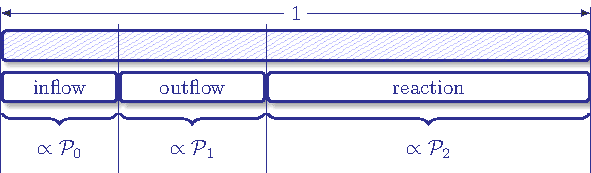
\includegraphics[width=0.5\linewidth]{graphics/chapter6/rel_prob.pdf}
    \vspace{0.5cm}
    \caption{The calculation of the weights for choosing whether to effect an inflow, outflow or a reaction at a particular simulation step.}
    \label{fig:rel_prob}
\end{figure}

The possibility of mass flow in and out of the system not only allows for simulation of open systems, but also permits a given system to be studied under two possible conditions. Without mass flows, the system will converge towards a steady-state, in which the counts of the molecules of each class (which in turn determine the reactions occurring in the system, as discussed in Section~\ref{stocProcess}) make the number of molecules of each class produced by reactions balance the number consumed by reactions. This is analogous to the notion of equilibrium control~\cite{thermodynamic_control}. On the other hand, with mass flows the number of reactions required to form a molecule of given class becomes a major influence on its count in the system, since a longer pathway allows for more outflow of mass on which the molecule class depends. This is analogous to kinetic control~\cite{kinetic_control} in chemical systems.

\section{Algorithm}
\label{sec:algorithm}

The algorithm used to allow the system to evolve is presented in Algorithm~\ref{generate_network}. This adopts the discrete scheme of either mimicking a collision to effect a reaction, sampling some molecules to remove from the system or adding some more molecules to it at an iteration in the simulation. 
Effecting a reaction in the system is divided into three successive steps: choosing colliding molecular pair, choosing a reaction template, and subsequently, choosing a reaction instance from the enumerated reactions.
This leads to progressive exploration of the underlying reaction network described by the specified graph grammar (i.e., set of reaction templates and set of initial molecular graphs) as the simulation progresses.

\begin{algorithm}[!h]
    \caption{}
    \begin{footnotesize}
    \begin{algorithmic}[1]
        \State Input: 
        \State \hspace{1cm} initial state $s_0$
        \State \hspace{1cm} number of simulation steps $N$
        \State \hspace{1cm}  \texttt{get\_rxns} method returning reactions by applying a template to a pair of molecules
        \State \hspace{1cm} inflow vector $\delta$
        \State \hspace{1cm} stochastic rate constants $k_0$, $k_1$ and $k_2$
        \State $i \leftarrow 0$ 
        \State $s[i] \leftarrow s_0$
        \While{ $i \leq N$}
            \State i++
            \State \textcolor{gray}{calculate $\mathcal{P}_0$, $\mathcal{P}_1$ and $\mathcal{P}_2$ using \eqref{zero_order}, \eqref{first_order} and \eqref{second_order} \Comment{relative probabilities}}
            \State \textcolor{gray}{choose a random number $\rho \in [0,1)$}
            \If{\textcolor{gray}{$\rho < \mathcal{P}_0/\sum_{i=0}^2 \mathcal{P}_i$}} \textcolor{gray}{\Comment{inflow block}}
                \State \textcolor{gray}{$s[i+1] \leftarrow s[i] + \delta$ \Comment{add inflow}}
        	\ElsIf{\textcolor{gray}{$\rho < \left[\mathcal{P}_0 + \mathcal{P}_1\right]/\sum_{i=0}^2 \mathcal{P}_i$}} \textcolor{gray}{\Comment{outflow block}}
                \State \textcolor{gray}{choose $m$ from $s[i]$  \Comment{outflow candidate}}
        		\State \textcolor{gray}{assemble outflow $\epsilon = [m]$}
                \State \textcolor{gray}{$s[i+1] \leftarrow s[i] - \epsilon$} \textcolor{gray}{\Comment{subtract outflow}}
            \Else \Comment{collision-reaction block}
		    	\State choose $(m_1, m_2)$ from $s[i]$  \Comment{collision pair}
	        	\State choose $r$ from $R$ \Comment{reaction template}
	        	\State \texttt{rxns} = \texttt{get\_rxns}$(m_1, m_2, r)$\Comment{return possible reactions} 
		        \If{\texttt{rxns}.length $> 0$}
		    	    \State Choose a \texttt{rxn} (defining $\nu^-$ and $\nu^+$) out of \texttt{rxns} randomly
		    	    \State $s[i+1] \leftarrow s[i] - \nu^- + \nu^+$ \Comment{update the current state} 
		        \EndIf
            \EndIf
        \EndWhile
        \State return $s$
    \end{algorithmic}
    \end{footnotesize}
    \label{generate_network}
\end{algorithm}

The steps in gray in Algorithm~\ref{generate_network} are optional and concern the in- and outflow parts. They can be enabled if inflows and outflows are desired, or can be skipped altogether to simulate a closed system.

The selection of $m_1$ and $m_2$ in line~15 is done according to Equation~\eqref{react_prob_different_molecules} and ~\eqref{react_prob_same_molecules}. The selection of a reaction $j$ to execute is done in line~17 by the method \texttt{get\_rxns(),} which implements the two step process described in Section~\ref{reaction_enumerate}.

Note that the loop iterates over the collision numbers, and in each iteration an event (inflow, outflow, or a collision) is supposed to occur.
However, the collisions between the molecules do not occur at roughly equal intervals of time,
if the total number of molecules in the system changes and the simulations runs under constant volume conditions.
Considering the system to be an ideal gas (where all molecules are of the same size, and the total volume of the molecules is negligible compared to that of the gas),
the collision frequency depends on the number of molecular pairs in the system.
This disregards all collisions involving three of more molecules simultaneously (which is anyway rare).
Therefore, to keep track of the time, the time step has to be weighted by the number of molecular pairs in the system.
If the system started off with $N_0$ molecules initially, and has $N$ molecules at time $t$, then the increment in real time would be
\begin{equation*}
    t \leftarrow t + \Delta t \cdot \frac{N_0(N_0-1)}{N(N-1)}
\end{equation*}
or the time interval between two collision events scales inversely with the number of molecular pairs in the system. However, if the system is simulated under constant pressure conditions (as is the case in most natural situations), the volume of the system adjusts, keeping the collision frequency roughly unchanged.

\section{Experiments}
\label{exp}

In this section, we use the formose reaction as a case study to assess the behaviour of the exploration framework on a chemically rich generative system. The purpose of these experiments is not to validate quantitative reaction kinetics, since the method does not aim to reproduce them, but to examine which regions of the reachable molecular space are discovered under different exploration conditions and how open-system dynamics affect that discovery process. We therefore analyse observables such as molecular-size distributions, diversity of molecular classes, innovation of newly encountered molecules, and the abundances of selected biologically relevant products~\cite{formose_prebiotic}. These observables characterize the exploratory trajectory induced by the sampling policy and illustrate the kinds of chemically interpretable questions the framework can address.

Simulations to study the formose reaction network were carried out under two conditions: a closed system and a system with inflows and outflows. In the flow-enabled case, the fixed inflow vector $\delta$ consisted of methanal only.
We initialized the system with $990$ molecules of methanal and $10$ molecules of 2-hydroxyethanal ($1 \%$ mol) when flows were disabled. When flows were allowed, $10$ molecules of 2-hydroxyethanal were found to not have the sufficient catalytic activity for the system to evolve, as all these molecules were often removed by outflow steps even before they could react with methanal. Therefore, we initialized the system with $950$ molecules of methanal and $50$ molecules of 2-hydroxyethanal ($5 \%$ mol), that is, with a higher number of catalyst molecules, when flows were allowed. The reaction templates consisted of the reaction templates for keto–enol tautomerism, aldol addition, and their reverse reactions. Graph representations of molecules do not encode stereochemistry; therefore, all aldopentose stereoisomers (arabinose, lyxose, ribose, and xylose) are represented by isomorphic graphs. In both cases, the simulation consisted of $10^6$ iteration steps, and equilibrium was operationally defined as the point at which each molecular count became stable.

\begin{figure}[!b]
    \centering
    \begin{subfigure}{0.45\textwidth}
        \centering
        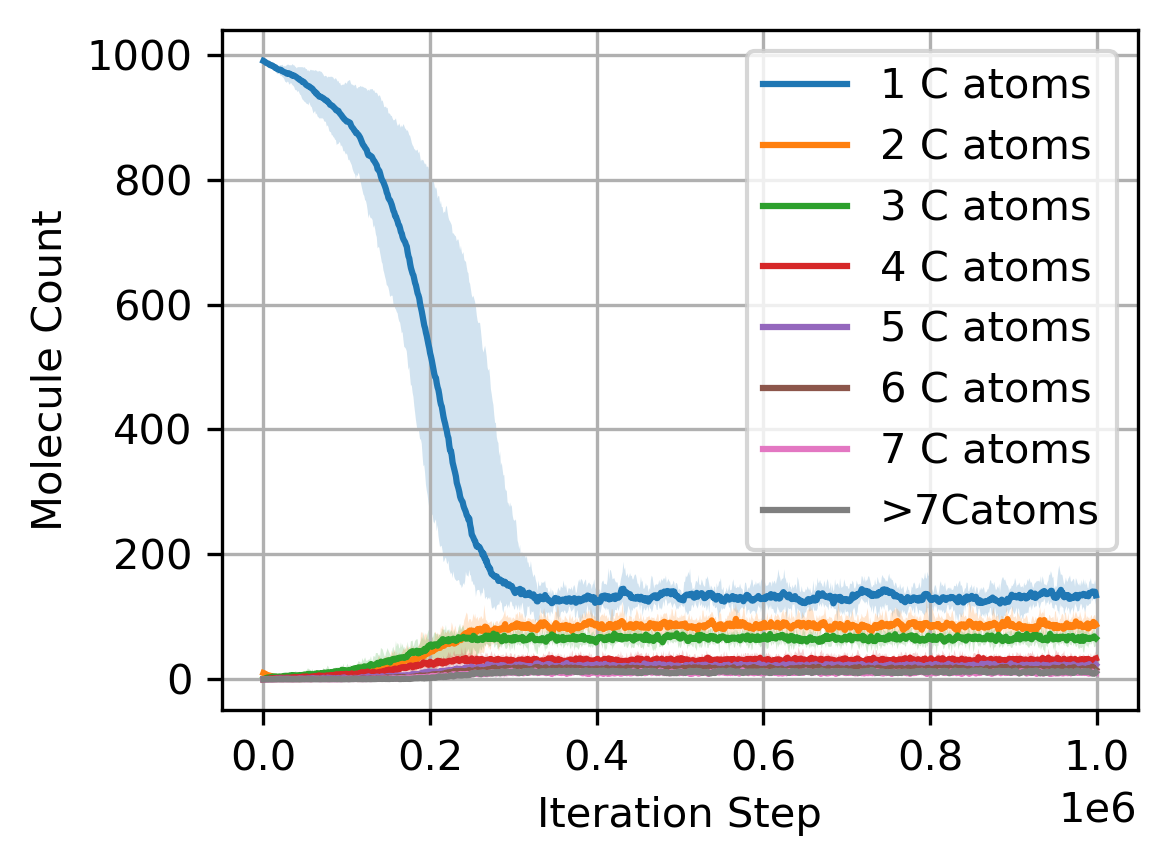
\includegraphics[width=\textwidth]{graphics/chapter6/numMolsNoFlow.png}
        \caption{In the closed system, larger molecules are formed . See also Figure~\ref{fig:distMolsNoFlowZoom} for a zoomed-in view.}
        \label{fig:distMolsNoFlow}
    \end{subfigure}% 
    \hfill
    \begin{subfigure}{0.45\textwidth}
        \centering
        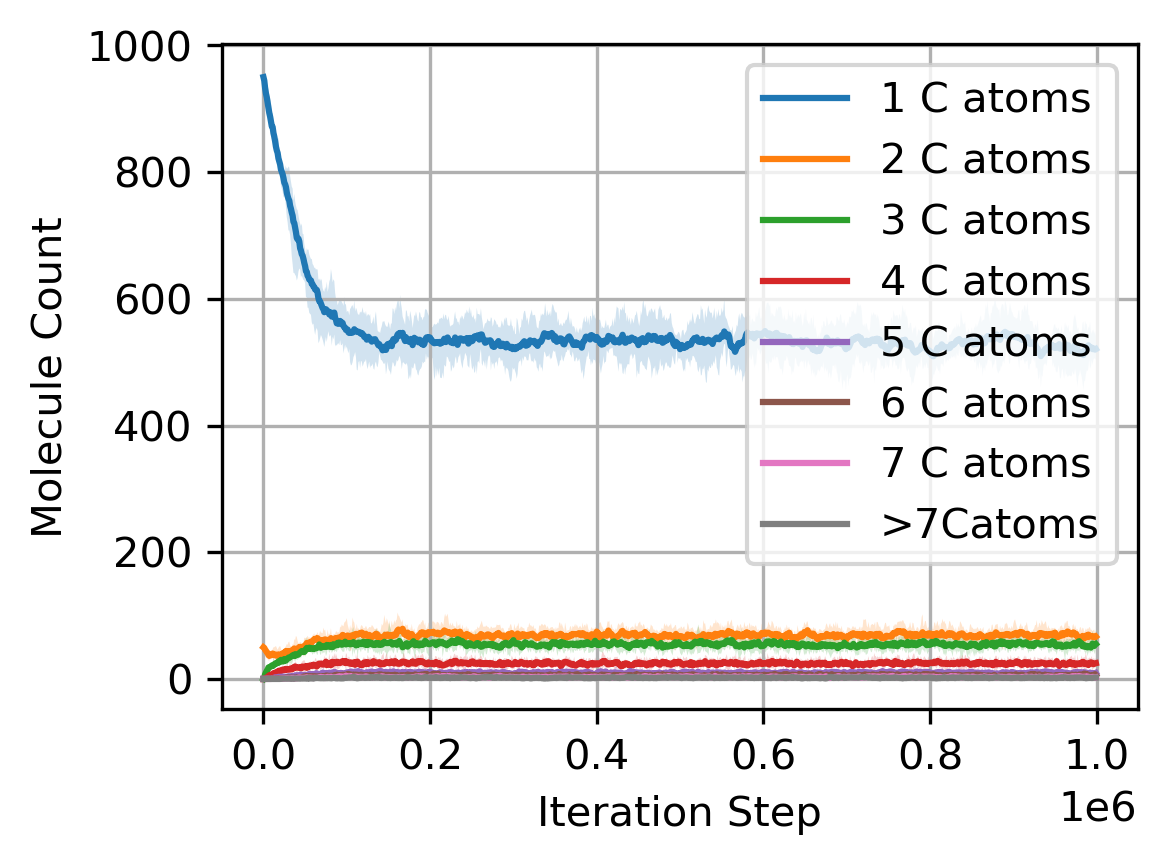
\includegraphics[width=\textwidth]{graphics/chapter6/numMolsFlow.png}
        \caption{In the flow-enabled system, smaller molecules are more abundant. See also Figure~\ref{fig:distMolsFlowZoom} for a zoomed-in view.}
        \label{fig:distMolsFlow}
    \end{subfigure}
    \\
    \vspace{0.8cm}
    \begin{subfigure}{0.45\textwidth}
        \centering
        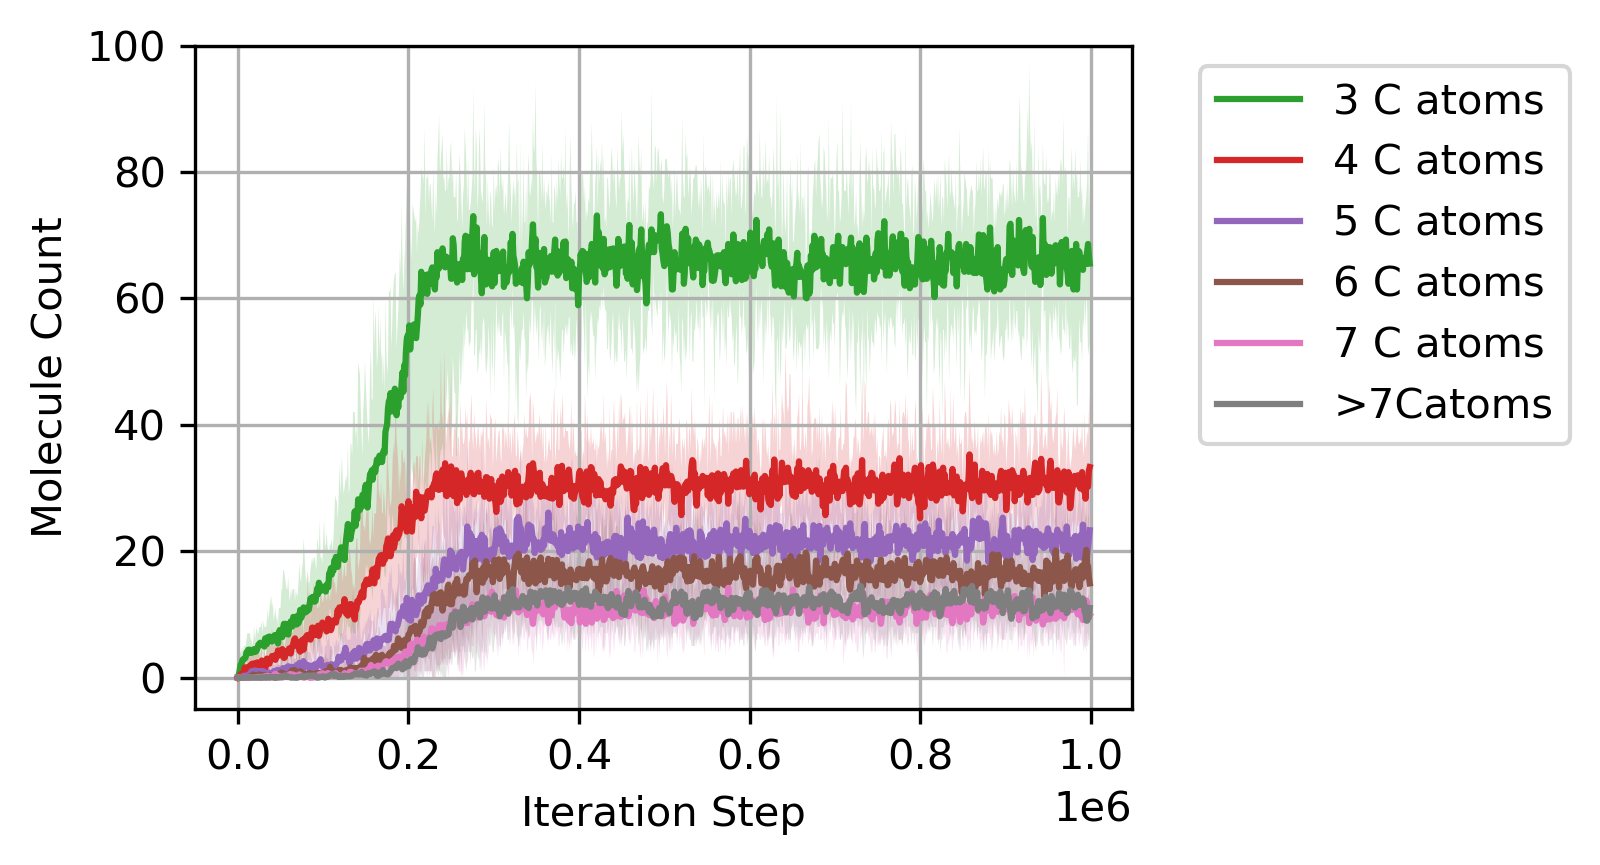
\includegraphics[scale=0.5]{graphics/chapter6/numMolsNoFlow_3_7.png}
        \caption{A zoomed-in part of Figure~\ref{fig:distMolsNoFlow} showing the molecules with five, six or more carbon atoms are more abundant than Figure~\ref{fig:distMolsFlowZoom}.}
        \label{fig:distMolsNoFlowZoom}
    \end{subfigure}% 
    \hfill
    \begin{subfigure}{0.45\textwidth}
        \centering
        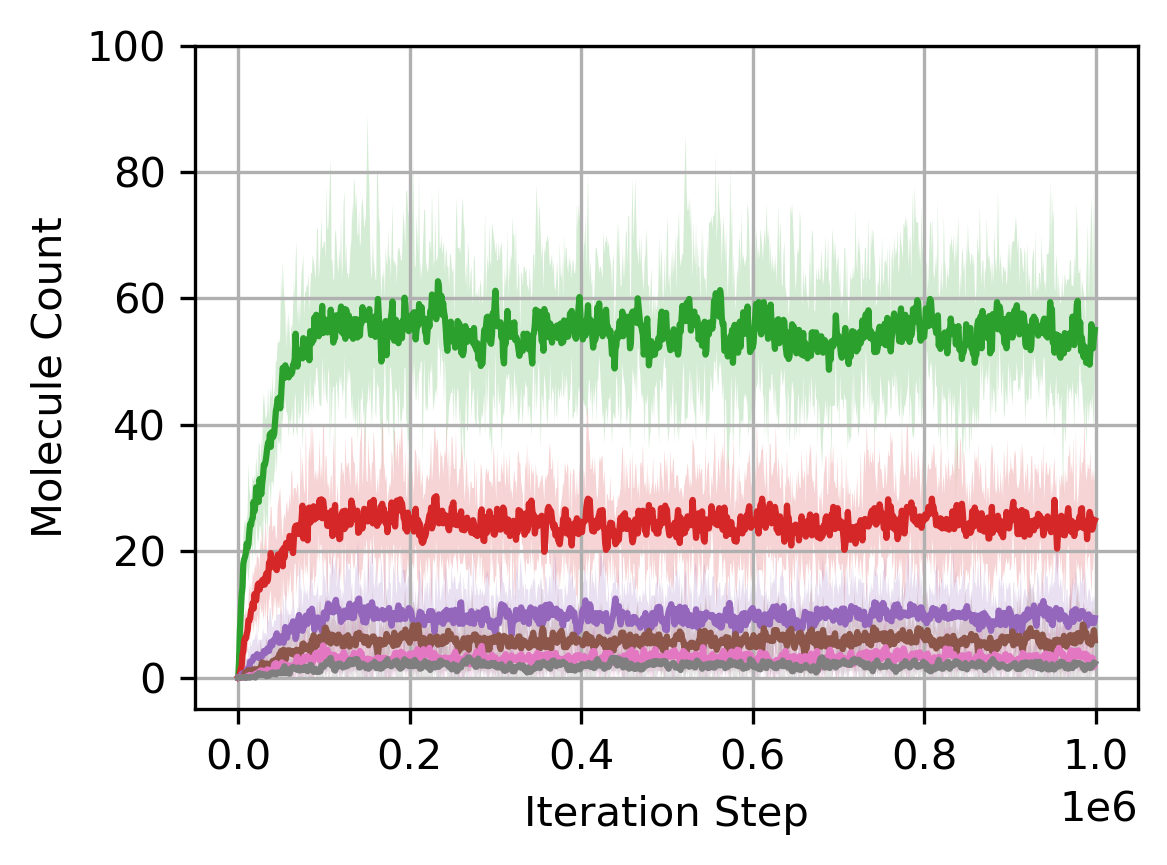
\includegraphics[scale=0.5]{graphics/chapter6/numMolsFlow_3_7.png}
        \caption{A zoomed-in part of Figure~\ref{fig:distMolsFlow} showing the molecules with five, six or more carbon atoms are less abundant than Figure~\ref{fig:distMolsNoFlowZoom}.}
        \label{fig:distMolsFlowZoom}
    \end{subfigure}
    \vspace{0.5cm}
    \caption{The plots show the evolution of the numbers of molecules of different sizes during the simulation. If there are multiple classes of molecules with the same number of carbon atoms, they are summed up and the mean total count of molecules with a particular number of carbon atoms is plotted. All molecules with more than $7$ carbon atoms are lumped in a single bin. The values plotted are averages over $100$ trials and the shaded region around a solid curve shows the standard deviation.}
    \label{fig:distMols}
\end{figure}
Figure~\ref{fig:distMols} summarizes the evolution of molecule counts by carbon number for each scenario, with the closed system shown in Figure~\ref{fig:distMolsNoFlow} and Figure~\ref{fig:distMolsNoFlowZoom} and the flow-enabled system in Figure~\ref{fig:distMolsFlow} and Figure~\ref{fig:distMolsFlowZoom}.

The total number of carbon atoms in the closed system should of course remain constant (at the initial value of $1010$) throughout the simulation. This is also what was observed, as shown in Figure~\ref{fig:massMols}. Because all molecules generated from the reaction templates conform to the empirical formula (CH$_2$O)$_n$, the system’s mass can be inferred by multiplying the carbon count by $(12+16+2\times 1) = 30$. For the open system, inflow and outflow rates were tuned such that the mean total carbon count throughout the simulation remained close to the initial value of $950 + 2 \times 50 = 1050$. This maintained it close to that of the closed system, allowing for direct comparison without confounding effects from differences in system size. To accomplish this, the inflow stochastic rate constant was set to $k_0 = 75$, and the outflow stochastic rate constant to $k_1 = 0.1$. Across $100$ runs, the mean number of carbon atoms in the open system was $1055$, with a standard deviation of $43$, as depicted in Figure~\ref{fig:massMols}.

Because methanal is the overwhelmingly dominant species in both scenarios, the total number of molecules largely tracks the methanal count. In the closed system, the total population stabilizes at $\sim 375\pm 15$ after $4\times 10^5$ simulation steps, whereas in the open system it stabilizes around $\sim 700\pm 25$ after $2\times 10^5$ simulation steps. The number of molecules in the system is higher when flows are enabled as molecules are replenished by the inflow of methanal, and it stabilizes quicker than in the closed system. The total molecule count is lower in the closed system because carbon atoms accumulates in larger molecules without the possibility of replenishment.
\begin{figure}
    \centering
    \begin{subfigure}{0.45\textwidth}
        \centering
        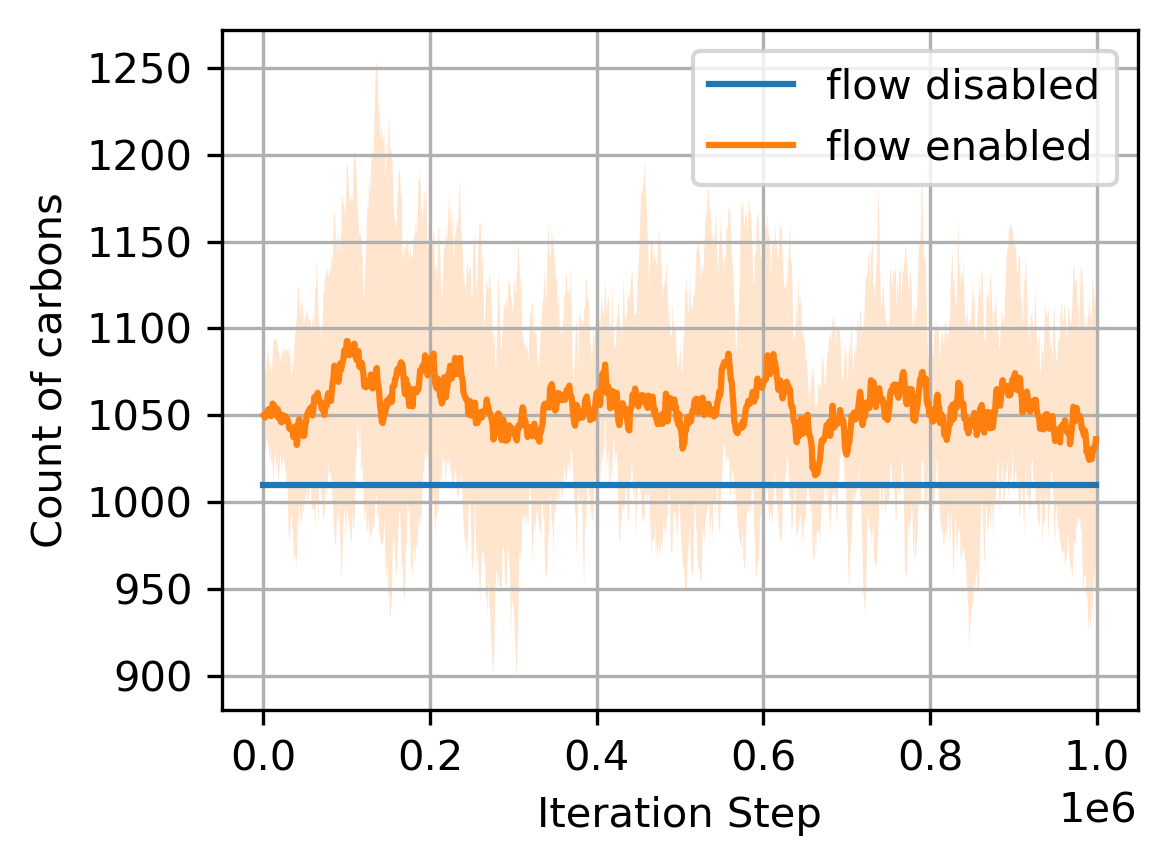
\includegraphics[width=\textwidth]{graphics/chapter6/numCarbons.png}
        \caption{Number of carbons in the system.}
        \label{fig:massMols}
    \end{subfigure}% 
    \hfill
    \begin{subfigure}{0.45\textwidth}
        \centering
        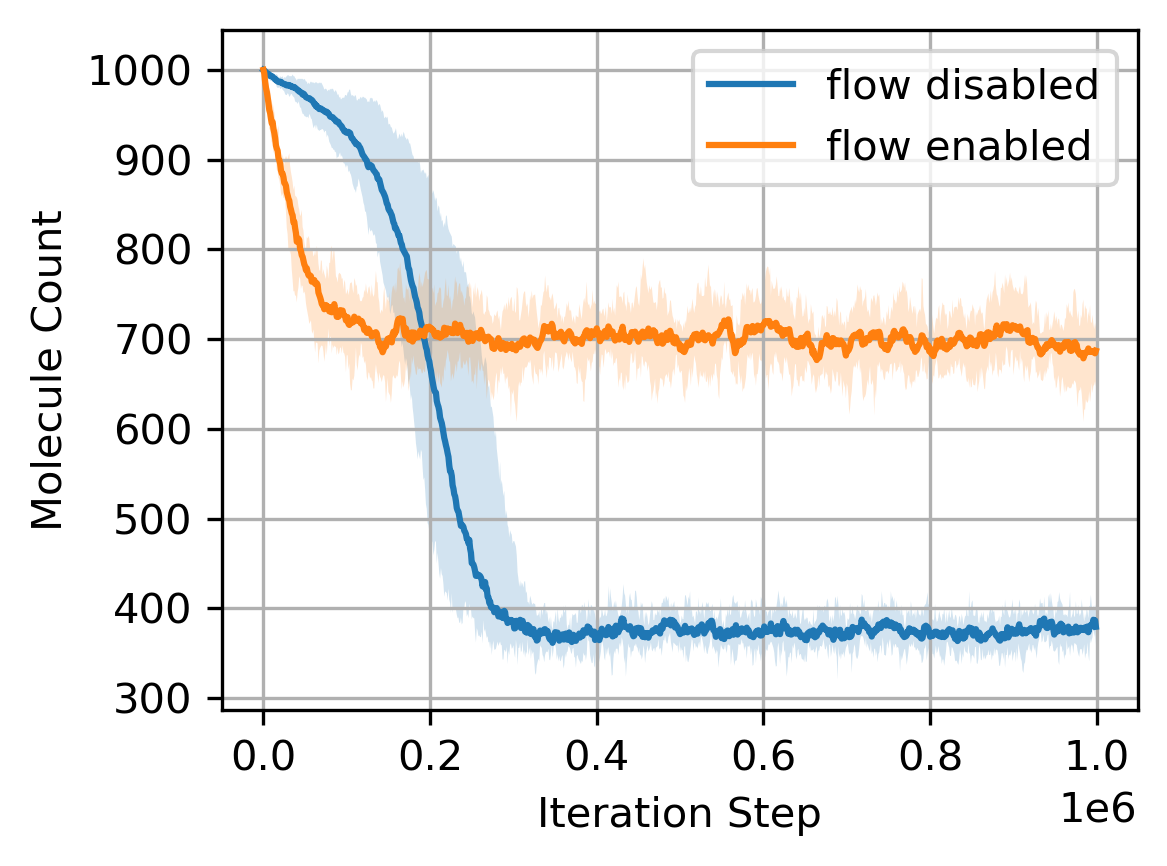
\includegraphics[width=\textwidth]{graphics/chapter6/numMols.png}
        \caption{Number of molecules in the system.}
        \label{fig:numMols}
    \end{subfigure}
    \\
    \vspace{1.0cm}
    \begin{subfigure}{0.45\textwidth}
        \centering
        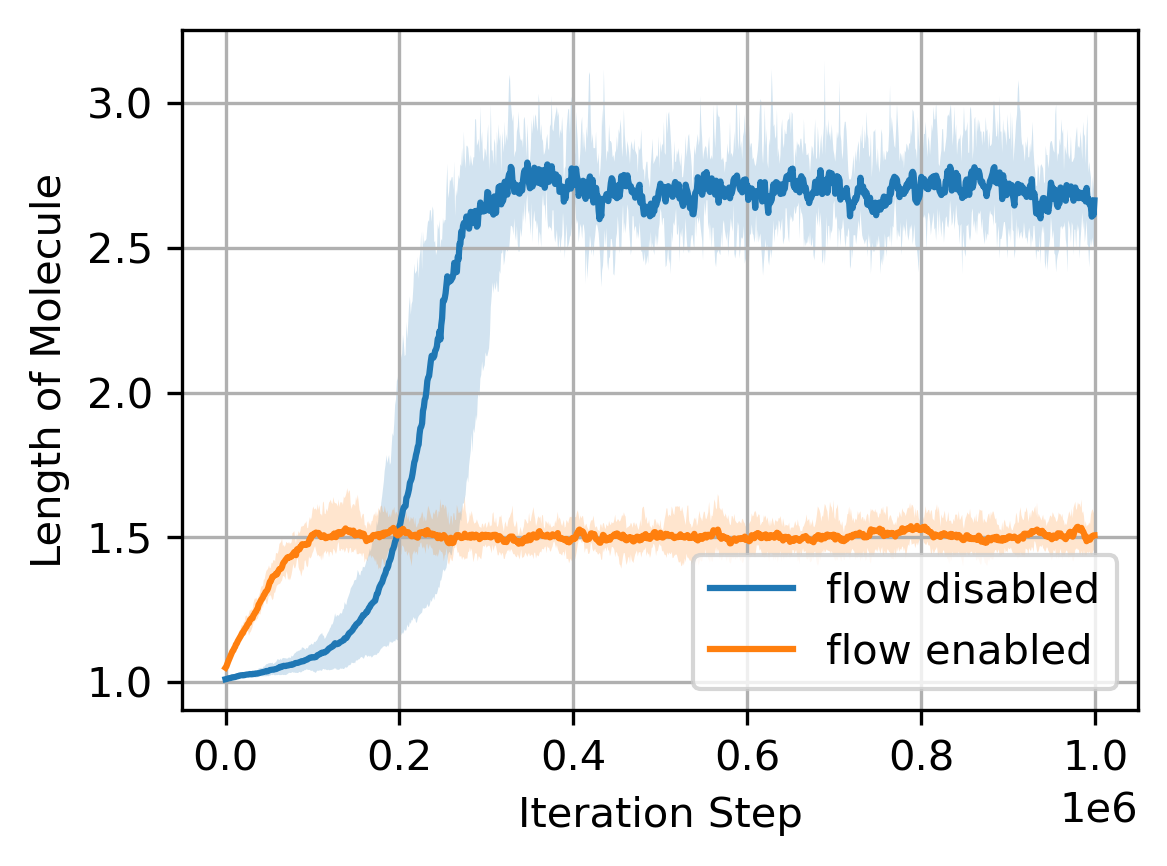
\includegraphics[width=\textwidth]{graphics/chapter6/avgMolLength.png}
        \caption{Average length of a molecule in the system.}
        \label{fig:lenMols}
    \end{subfigure}% 
    \hfill
    \begin{subfigure}{0.45\textwidth}
        \centering
        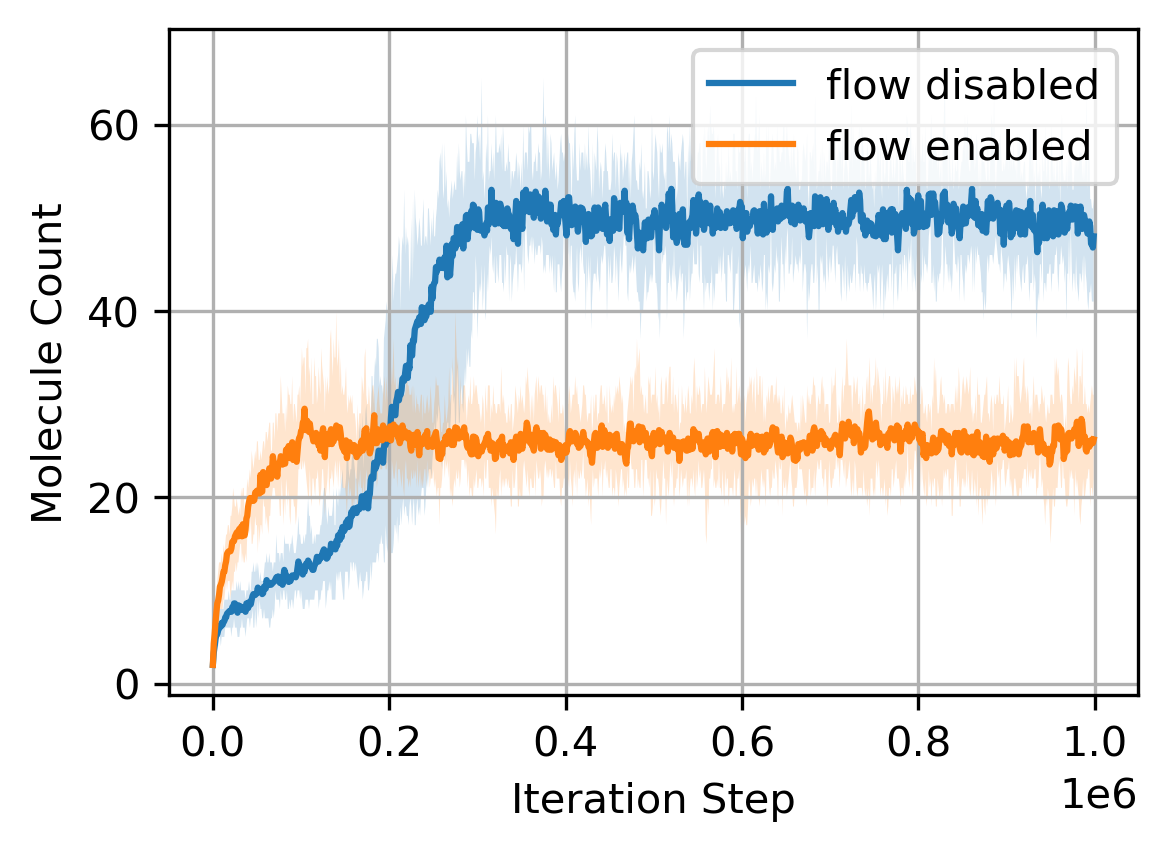
\includegraphics[width=\textwidth]{graphics/chapter6/uniqueMols.png}
        \caption{Number of distinct classes of molecules.}
        \label{fig:uniqueMols}
    \end{subfigure}
    \\
    \vspace{1.0cm}
    \begin{subfigure}{0.45\textwidth}
        \centering
        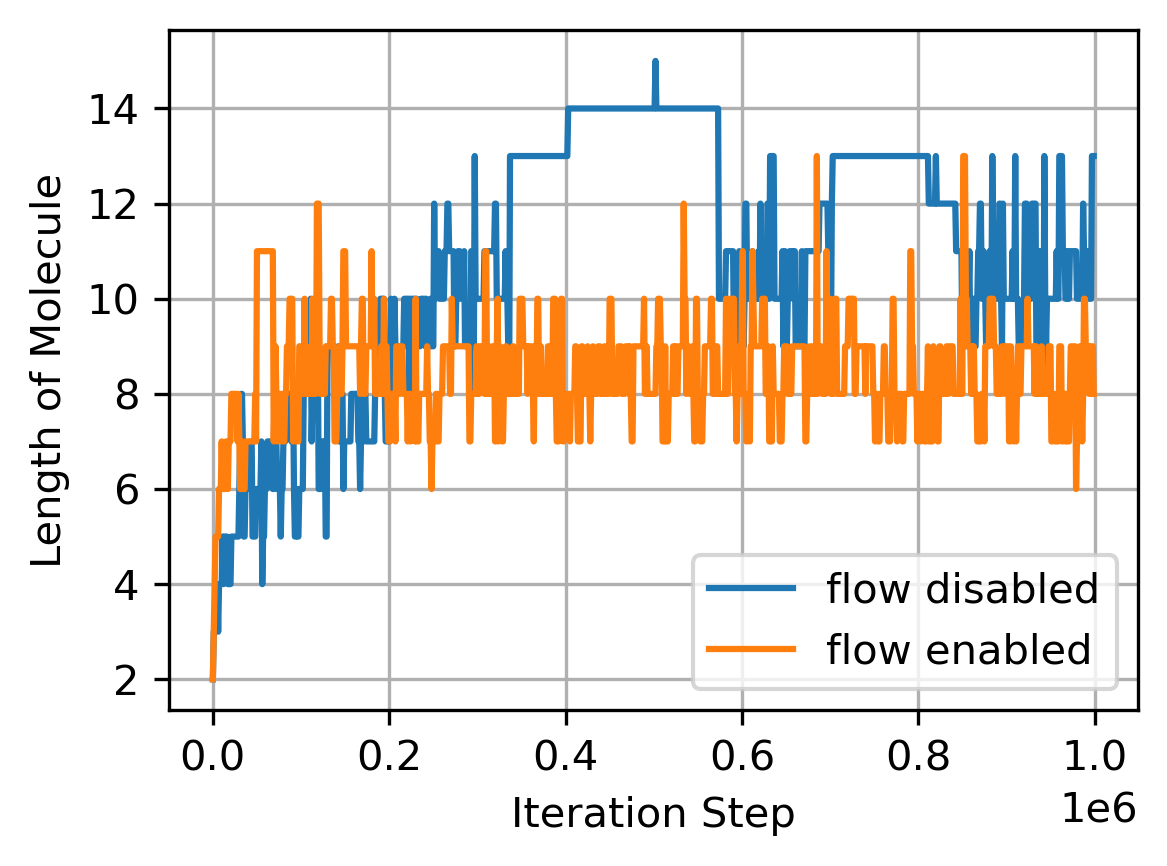
\includegraphics[width=\textwidth]{graphics/chapter6/longestMol.png}
        \caption{Length of the longest molecule in the system.}
        \label{fig:maxLenMols}
    \end{subfigure}% 
    \hfill
    \begin{subfigure}{0.45\textwidth}
        \centering
        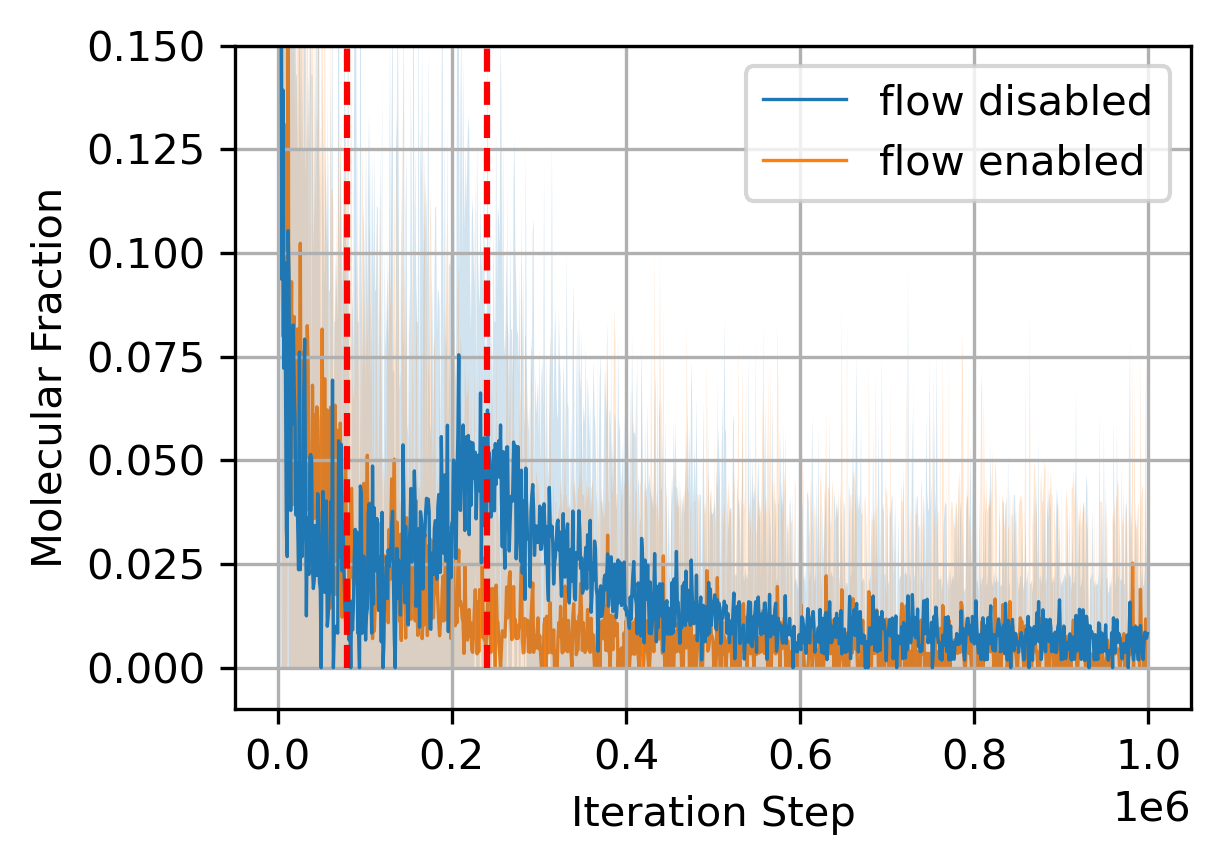
\includegraphics[width=\textwidth]{graphics/chapter6/newMols.png}
        \caption{Fraction of new molecules.}
        \label{fig:newMols}
    \end{subfigure}
    \vspace{0.5cm}
    \caption{Some parameters describing the system when the system is closed and when there is flow into and out of the system. The solid lines show the mean values and the shaded regions show the standard deviation, both over $100$ runs.}
    \label{fig:propMols}
\end{figure}

The average molecular length (defined as the average number of carbon atoms in the molecule) differs markedly between the two conditions, as seen in Figure~\ref{fig:lenMols}. In the closed system, the average stabilizes at roughly three carbons (with mean $2.7$ and standard deviation $0.1$). In the closed system, methanal can readily be consumed to form larger molecules which raises the average length of the molecule. In the open system, however, the average settles at the lower value of $1.5$ with a standard deviation of less than $0.05$. This was to be expected: outflow tends to remove molecules before they can react to form longer molecules, while continual methanal inflow persistently skews the distribution toward shorter molecules.

The number of unique molecules—defined as the number of distinct molecular graphs in the system at any given time—diverges significantly across the two regimes (as shown in Figure~\ref{fig:numMols}). In the closed system, this count rises rapidly after an initial lag phase (the first $2\times 10^5$ simulation steps) and plateaus near $\sim 50\pm 4$. In the open system, the number of distinct molecules increases from the start and is higher than that in the closed system initially. However, the number stabilizes to a lower value of $\sim 26\pm 3$ after around $2\times 10^5$ simulation steps. This difference reflects the underlying population dynamics. In the closed system, new molecules typically arise from existing ones, since even molecular classes with few instances can react to form molecules from new classes. In contrast, the continuous outflow of molecules removes classes of molecules with more carbon atoms entirely from the system. This prevents them from forming larger and more complex counterparts, leading to a lower number of unique molecules in the system. This lower number of distinct molecular classes in the open system combined with the observation from Figure~\ref{fig:numMols} that the total number of molecules is higher implies that there are more copies of molecules of each class (in particular methanal) when flows are allowed.

Figure~\ref{fig:maxLenMols} traces the length of the longest molecule (defined as the number of carbon atoms in the molecular class with the maximum number of carbon atoms) over the progress of the simulation. Because this metric is highly sensitive to single fragmentation or condensation reaction events, the figure shows data from a single representative run of the simulation rather than the mean over multiple trials—averaging would obscure the abrupt jumps that characterize this quantity. Long molecules can fragment suddenly into much smaller species, or moderate-sized molecules can condense into substantially larger ones, producing large fluctuations in this measure. The conclusion that might be drawn is that when flows are enabled, the length of the longest molecule in the system is smaller compared to when the system is closed. Initially, the length of the longest molecule is higher in the system when flows are allowed, but as the closed system enters the generative phase (after the first $2\times 10^5$ simulation steps), the longest molecule in the closed system has a more carbon atoms.

Figure~\ref{fig:newMols} shows the innovation rate, defined as the fraction of molecular classes at simulation step~$i$ that were absent in all of the previous~$i-1$ steps:
\begin{equation*}
    \text{innovation rate} = \frac{\text{number of molecular classes not in previous $i-1$ steps}}{\text{number of molecular classes in step }i}
\end{equation*}
Because the molecular network is explored through a stochastic strategy, tracking newly discovered molecules provides insight into how effectively the simulation samples the accessible chemical space. If the innovation rate were to reach zero, the system would no longer generate new molecular structures, indicating that probably the reachable portion of the network had been exhausted. Although the theoretical space of accessible molecules is unbounded, in practice very large molecules form only sporadically and are prone to fragmentation. Even in natural chemistry, monosaccharides larger than seven carbons are rarely observed (ignoring polymeric carbohydrates). So as the simulation progresses, the innovation rate should decrease gradually as more of the reachable molecular space is discovered and becomes a part of the already explored network, yet the system continues to operate in a quasi-generative regime.

In the closed system, a transient rise in innovation rate occurs between $\sim 0.8\times 10^5$ and $\sim 2.4\times 10^5$ steps, coinciding with the sharp increase in the number of unique molecules (in Figure~\ref{fig:uniqueMols}), the average length of the molecule (in Figure~\ref{fig:lenMols}) and the rapid decline in the number of methanal molecules. This generative phase in the simulation of the closed system is in Figure~\ref{fig:newMols} marked by the vertical dotted red lines. After this point, the number of new molecular classes generated becomes small but non-zero, as seen by the observed gradual decay in the innovation rate.
When flows are enabled, this generative phase does not appear in the simulation, and the innovation rate monotonically decreases as the simulation progresses.

\section{Suggested Improvements}

Several directions exist for improving the physical fidelity and computational efficiency of the framework:
\begin{enumerate}
    \item \emph{Kinetically informed sampling}: The two random-choice steps for selecting reaction templates and instances are intentionally simplified. A more realistic dynamics would incorporate reaction probabilities derived from the law of mass action, which requires rate constants (requiring estimates of activation energy barriers). Although computing these quantities is challenging, incorporating them would be necessary for recovering quantitatively accurate kinetics rather than purely exploratory behaviour. We expect caching reaction instances along with their energy barriers would significantly reduce the computation and speed up the simulation. Most simulation algorithms utilize educated guesses for the rate constants, which makes the behaviour of the system particularly sensitive to the inputs for these parameters. 
    \item \emph{Free Energy difference weighted instance selection}:
    	As a less ambitious alternative, reaction instance selection could use a Metropolis Hastings type acceptance rule (which is often used in high dimensional systems).
    	We sketch a possible scheme using weights of the form $\exp(-E_i/(\alpha k_B T))$ in Figure~\ref{fig:reac_mh_prob}, where $E_i$ is the free energy difference associated with the products of the $i$th candidate reaction and $\alpha$ is a parameter to adjust the relative probabilities of the candidate reactions. While such weights resemble those used in equilibrium sampling (e.g., grand canonical ensembles) in thermodynamic Monte Carlo simulations, adapting them to chemical kinetic transitions may offer a controllable bias with reaction pathways towards energetically favourable regions of the network. Moreover, in simulations to elucidate the equilibrium state through Monte Carlo simulations, the energy $E_i$ used in the acceptance rule is the free energy of the sampled state, and not the difference in free energies of two states.

    \begin{figure}
        \centering
        \vspace{0.5cm}
        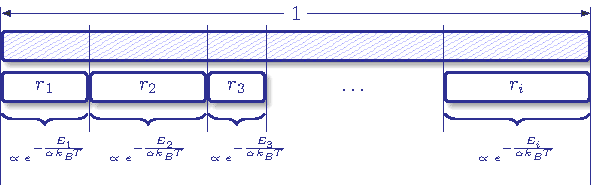
\includegraphics[width=0.5\linewidth]{graphics/chapter6/reac_mh_prob.pdf}
        \vspace{0.5cm}
        \caption{The calculation of the weights using a Metropolis-Hastings-type scheme after applying a reaction template to the selected pair of molecules generating the reactions $\{r_1, r_2, r_3, \cdots r_i\}$.}
        \label{fig:reac_mh_prob}
    \end{figure}
    
    \item \emph{Pathway tracing and caching strategies}: Many scientific questions, such as identifying plausible formation pathways from input molecules for queried molecules, require keeping track of reaction provenance. Alternative caching strategies can be investigated to quantify the speed-up they provide to the simulation and select the subspace of the implicit network explored by the algorithm. More sophisticated caching, indexing, or provenance-tracking structures could be developed depending on the needs of the study.
    \item \emph{Spatio-temporal simulations}: The framework can be naturally extended to simulate systems that are not well mixed by partitioning the volume or surface into multiple coupled regions (possibly arranged on a lattice). Each region hosts an independent instance of the stochastic simulation, while diffusion is modelled as inflow-outflow events between adjacent regions. This enables the study of systems with spatial heterogeneity emerging from the coupling of stochastic kinetics with diffusive transport. This allows investigation of concentration gradients, travelling waves, and oscillations, which arise in chemical systems with feedback loops and nonlinear kinetics.
    
    Coupling generative, rule-based frameworks with spatial discretization allows local differences in the exploration of the reaction network while permitting mass exchange between them. This opens the possibility of studying how spatial constraints influence molecular diversity, and the emergence of phenomena that are difficult to capture in well-mixed models: localized accumulation and shielding of molecules from dilution, or enabling compartmentalized autocatalysis. This broadens the applicability of the framework to heterogeneous environments on films, membranes, microfluidics, and early-earth or extraterrestrial settings.
\end{enumerate}
The continuation of this work will focus on incorporating these refinements in order to increase both accuracy and scalability of the algorithm for the exploration of large reaction networks. By combining template-based modelling with stochastic exploration, the framework opens a path toward systematically probing large reaction networks that are otherwise difficult to enumerate or simulate with conventional deterministic or kinetics-driven methods. 

